\documentclass{standalone}
\usepackage{tikz}
\usetikzlibrary{patterns, positioning}
\usepackage[sfdefault]{ClearSans} %% option 'sfdefault' activates Clear Sans as the default text font
\usepackage[T1]{fontenc}

\begin{document}
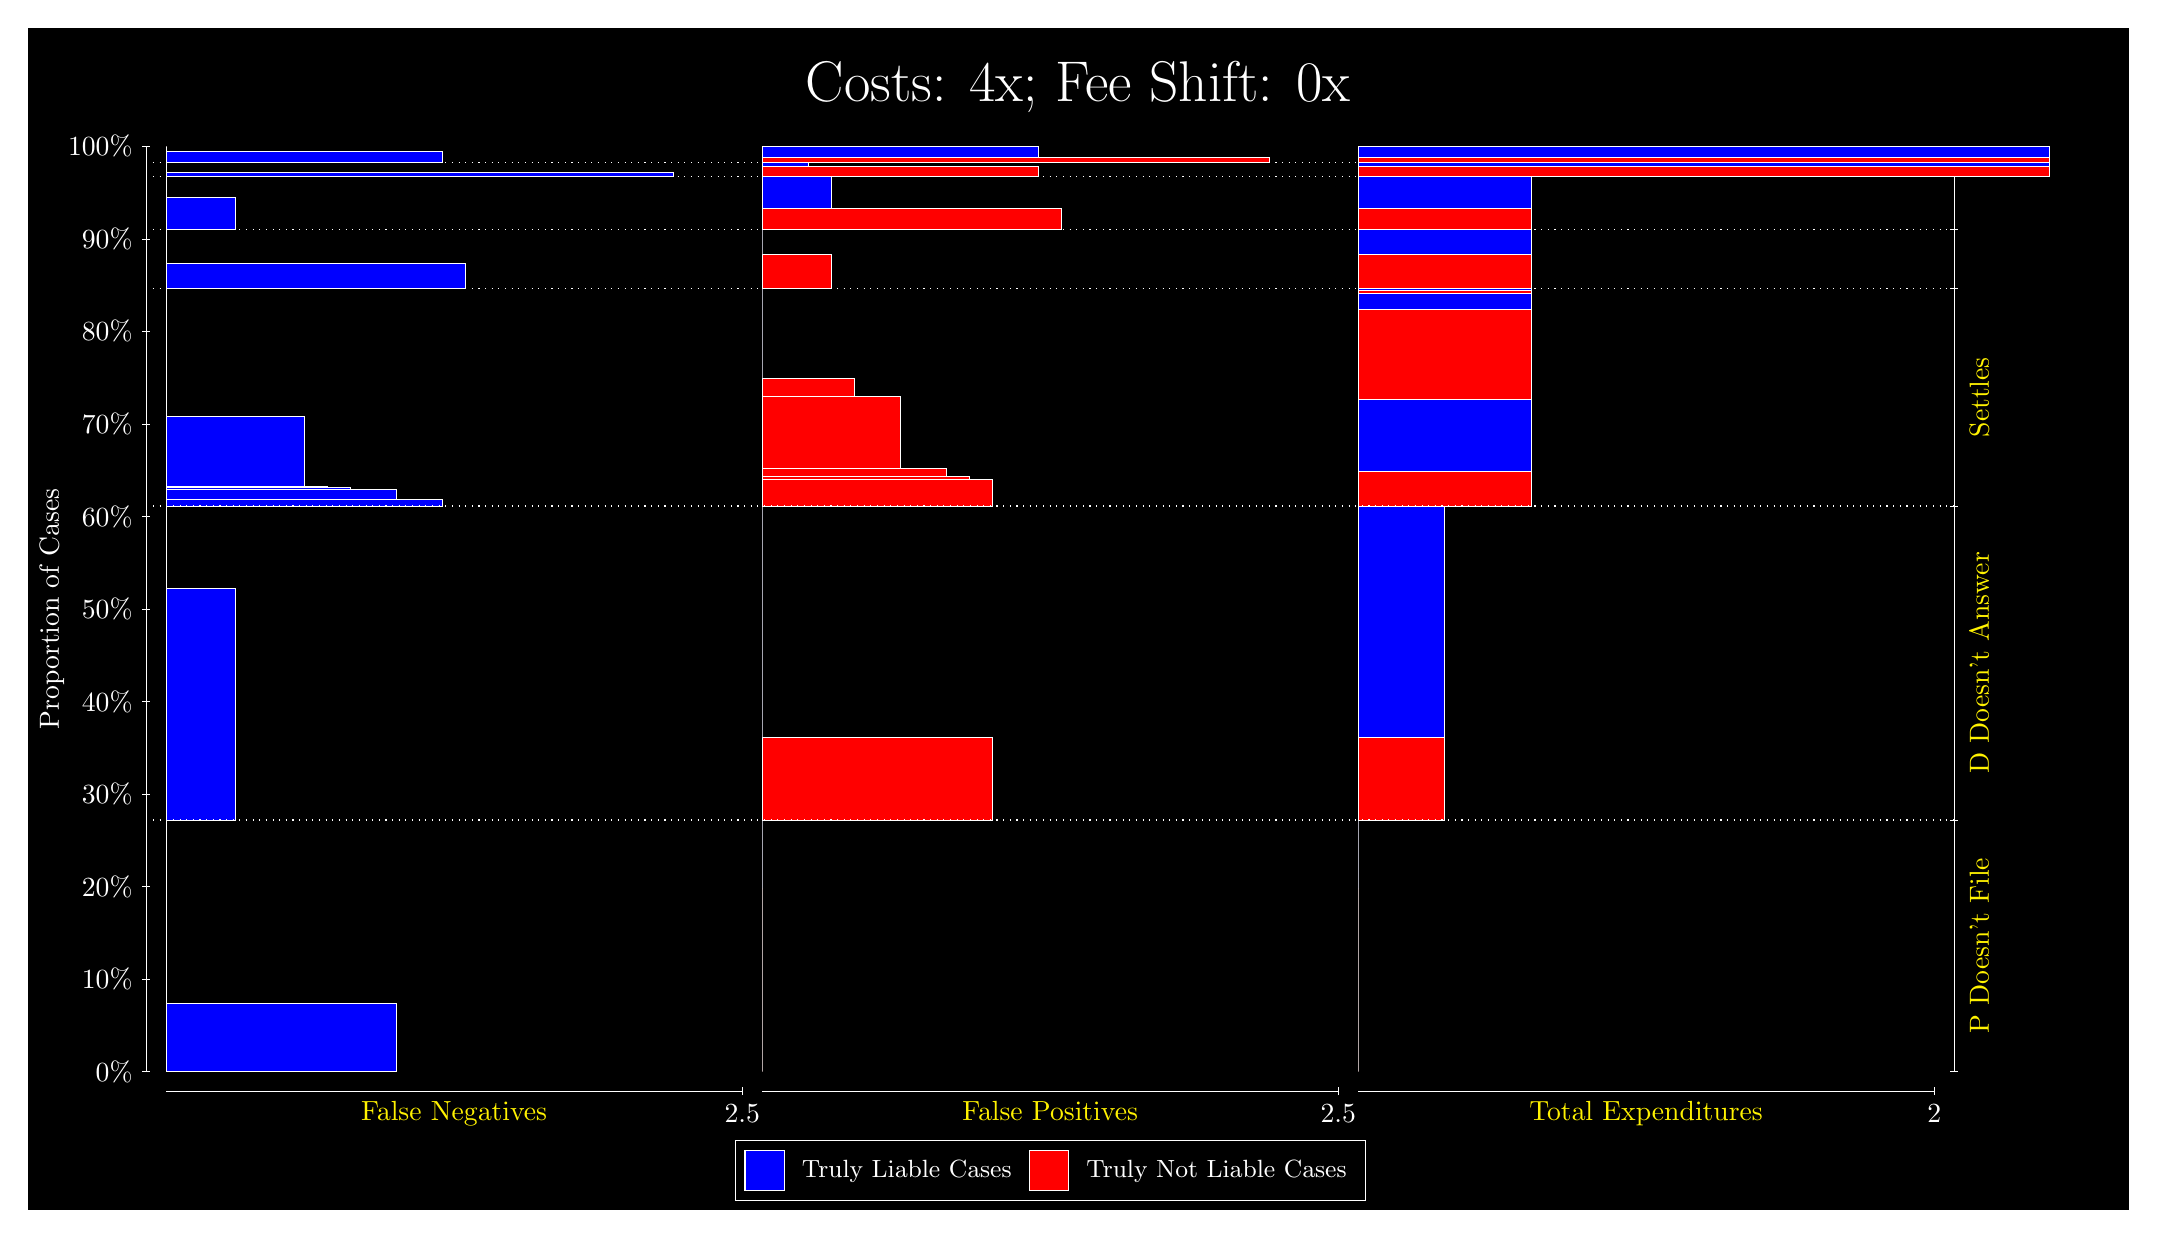
\begin{tikzpicture}
\draw[fill=black] (0,0) rectangle (26.667,15);
\draw[text=white] (0,13.5) rectangle (26.667,15) node[midway] {\huge Costs: 4x; Fee Shift: 0x};
\draw[white, very thin] (1.5,1.75) -- (1.5,13.5);
\node[rotate=90, text=white, anchor=center] at (0.3, 7.625) {Proportion of Cases};
\draw[white, very thin] (1.45,1.75) -- (1.55,1.75);
\node[text=white, anchor=east] at (1.45, 1.75) {0\%};
\draw[white, very thin] (1.45,2.925) -- (1.55,2.925);
\node[text=white, anchor=east] at (1.45, 2.925) {10\%};
\draw[white, very thin] (1.45,4.1) -- (1.55,4.1);
\node[text=white, anchor=east] at (1.45, 4.1) {20\%};
\draw[white, very thin] (1.45,5.275) -- (1.55,5.275);
\node[text=white, anchor=east] at (1.45, 5.275) {30\%};
\draw[white, very thin] (1.45,6.45) -- (1.55,6.45);
\node[text=white, anchor=east] at (1.45, 6.45) {40\%};
\draw[white, very thin] (1.45,7.625) -- (1.55,7.625);
\node[text=white, anchor=east] at (1.45, 7.625) {50\%};
\draw[white, very thin] (1.45,8.8) -- (1.55,8.8);
\node[text=white, anchor=east] at (1.45, 8.8) {60\%};
\draw[white, very thin] (1.45,9.975) -- (1.55,9.975);
\node[text=white, anchor=east] at (1.45, 9.975) {70\%};
\draw[white, very thin] (1.45,11.15) -- (1.55,11.15);
\node[text=white, anchor=east] at (1.45, 11.15) {80\%};
\draw[white, very thin] (1.45,12.325) -- (1.55,12.325);
\node[text=white, anchor=east] at (1.45, 12.325) {90\%};
\draw[white, very thin] (1.45,13.5) -- (1.55,13.5);
\node[text=white, anchor=east] at (1.45, 13.5) {100\%};

\draw[white, very thin] (24.457,1.75) -- (24.457,13.5);
\draw[white, very thin] (24.407,1.75) -- (24.507,1.75);
\node[anchor=west] at (24.407, 1.75) {};
\draw[white, very thin] (24.407,4.9446) -- (24.507,4.9446);
\node[anchor=west] at (24.407, 4.9446) {};
\draw[white, very thin] (24.407,8.9315) -- (24.507,8.9315);
\node[anchor=west] at (24.407, 8.9315) {};
\draw[white, very thin] (24.407,11.695) -- (24.507,11.695);
\node[anchor=west] at (24.407, 11.695) {};
\draw[white, very thin] (24.407,12.445) -- (24.507,12.445);
\node[anchor=west] at (24.407, 12.445) {};
\draw[white, very thin] (24.407,13.117) -- (24.507,13.117);
\node[anchor=west] at (24.407, 13.117) {};
\draw[white, very thin] (24.407,13.298) -- (24.507,13.298);
\node[anchor=west] at (24.407, 13.298) {};
\draw[white, very thin] (24.407,13.5) -- (24.507,13.5);
\node[anchor=west] at (24.407, 13.5) {};

\draw[white, very thin, fill=blue] (1.75,1.75) rectangle (4.6775,2.6154);
\draw[white, very thin, fill=red] (1.75,2.6154) rectangle (1.75,4.9446);
\draw[white, very thin, fill=blue] (1.75,4.9446) rectangle (2.6283,7.8868);
\draw[white, very thin, fill=red] (1.75,7.8868) rectangle (1.75,8.9315);
\draw[white, very thin, fill=blue] (1.75,8.9315) rectangle (5.2631,9.0235);
\draw[white, very thin, fill=blue] (1.75,9.0235) rectangle (4.6775,9.1393);
\draw[white, very thin, fill=blue] (1.75,9.1393) rectangle (4.092,9.1636);
\draw[white, very thin, fill=blue] (1.75,9.1636) rectangle (3.7993,9.1839);
\draw[white, very thin, fill=blue] (1.75,9.1839) rectangle (3.5065,10.071);
\draw[white, very thin, fill=red] (1.75,10.071) rectangle (1.75,11.695);
\draw[white, very thin, fill=blue] (1.75,11.695) rectangle (5.5558,12.016);
\draw[white, very thin, fill=red] (1.75,12.016) rectangle (1.75,12.445);
\draw[white, very thin, fill=blue] (1.75,12.445) rectangle (2.6283,12.85);
\draw[white, very thin, fill=red] (1.75,12.85) rectangle (1.75,13.117);
\draw[white, very thin, fill=blue] (1.75,13.117) rectangle (8.1906,13.174);
\draw[white, very thin, fill=red] (1.75,13.174) rectangle (1.75,13.298);
\draw[white, very thin, fill=blue] (1.75,13.298) rectangle (5.2631,13.443);
\draw[white, very thin, fill=red] (1.75,13.443) rectangle (1.75,13.5);
\draw[white, very thin, fill=red] (9.3189,1.75) rectangle (9.3189,4.0792);
\draw[white, very thin, fill=blue] (9.3189,4.0792) rectangle (9.3189,4.9446);
\draw[white, very thin, fill=red] (9.3189,4.9446) rectangle (12.246,5.9893);
\draw[white, very thin, fill=blue] (9.3189,5.9893) rectangle (9.3189,8.9315);
\draw[white, very thin, fill=red] (9.3189,8.9315) rectangle (12.246,9.2778);
\draw[white, very thin, fill=red] (9.3189,9.2778) rectangle (11.954,9.3144);
\draw[white, very thin, fill=red] (9.3189,9.3144) rectangle (11.661,9.4155);
\draw[white, very thin, fill=red] (9.3189,9.4155) rectangle (11.075,10.325);
\draw[white, very thin, fill=red] (9.3189,10.325) rectangle (10.49,10.556);
\draw[white, very thin, fill=blue] (9.3189,10.556) rectangle (9.3189,11.695);
\draw[white, very thin, fill=red] (9.3189,11.695) rectangle (10.197,12.124);
\draw[white, very thin, fill=blue] (9.3189,12.124) rectangle (9.3189,12.445);
\draw[white, very thin, fill=red] (9.3189,12.445) rectangle (13.125,12.711);
\draw[white, very thin, fill=blue] (9.3189,12.711) rectangle (10.197,13.117);
\draw[white, very thin, fill=red] (9.3189,13.117) rectangle (12.832,13.241);
\draw[white, very thin, fill=blue] (9.3189,13.241) rectangle (9.9044,13.298);
\draw[white, very thin, fill=red] (9.3189,13.298) rectangle (15.759,13.355);
\draw[white, very thin, fill=blue] (9.3189,13.355) rectangle (12.832,13.5);
\draw[white, very thin, fill=red] (16.888,1.75) rectangle (16.888,4.0792);
\draw[white, very thin, fill=blue] (16.888,4.0792) rectangle (16.888,4.9446);
\draw[white, very thin, fill=red] (16.888,4.9446) rectangle (17.986,5.9893);
\draw[white, very thin, fill=blue] (16.888,5.9893) rectangle (17.986,8.9315);
\draw[white, very thin, fill=red] (16.888,8.9315) rectangle (19.083,9.3788);
\draw[white, very thin, fill=blue] (16.888,9.3788) rectangle (19.083,10.29);
\draw[white, very thin, fill=red] (16.888,10.29) rectangle (19.083,11.431);
\draw[white, very thin, fill=blue] (16.888,11.431) rectangle (19.083,11.638);
\draw[white, very thin, fill=red] (16.888,11.638) rectangle (19.083,11.675);
\draw[white, very thin, fill=blue] (16.888,11.675) rectangle (19.083,11.695);
\draw[white, very thin, fill=red] (16.888,11.695) rectangle (19.083,12.124);
\draw[white, very thin, fill=blue] (16.888,12.124) rectangle (19.083,12.445);
\draw[white, very thin, fill=red] (16.888,12.445) rectangle (19.083,12.711);
\draw[white, very thin, fill=blue] (16.888,12.711) rectangle (19.083,13.117);
\draw[white, very thin, fill=red] (16.888,13.117) rectangle (25.67,13.241);
\draw[white, very thin, fill=blue] (16.888,13.241) rectangle (25.67,13.298);
\draw[white, very thin, fill=red] (16.888,13.298) rectangle (25.67,13.355);
\draw[white, very thin, fill=blue] (16.888,13.355) rectangle (25.67,13.5);
\draw[white, dotted] (1.5,4.9446) -- (24.457,4.9446);
\draw[white, dotted] (1.5,8.9315) -- (24.457,8.9315);
\draw[white, dotted] (1.5,11.695) -- (24.457,11.695);
\draw[white, dotted] (1.5,12.445) -- (24.457,12.445);
\draw[white, dotted] (1.5,13.117) -- (24.457,13.117);
\draw[white, dotted] (1.5,13.298) -- (24.457,13.298);
\draw[white, very thin] (1.75,1.5) -- (9.0689,1.5);
\node[text=yellow, anchor=north] at (5.4094, 1.5) {False Negatives};
\draw[white, very thin] (9.0689,1.45) -- (9.0689,1.55);
\node[text=white, anchor=north] at (9.0689, 1.45) {2.5};

\draw[white, very thin] (9.3189,1.5) -- (16.638,1.5);
\node[text=yellow, anchor=north] at (12.978, 1.5) {False Positives};
\draw[white, very thin] (16.638,1.45) -- (16.638,1.55);
\node[text=white, anchor=north] at (16.638, 1.45) {2.5};

\draw[white, very thin] (16.888,1.5) -- (24.207,1.5);
\node[text=yellow, anchor=north] at (20.547, 1.5) {Total Expenditures};
\draw[white, very thin] (24.207,1.45) -- (24.207,1.55);
\node[text=white, anchor=north] at (24.207, 1.45) {2};

\node[text=yellow, centered, rotate=90] at (24.777, 3.3473) {P Doesn't File};
\node[text=yellow, centered, rotate=90] at (24.777, 6.938) {D Doesn't Answer};
\node[text=yellow, centered, rotate=90] at (24.777, 10.313) {Settles};





\draw (12.978300999999998,1.5) node[draw=none] (baseCoordinate) {};
\begin{scope}[align=center]
        \matrix[scale=0.5, draw=white, below=0.5cm of baseCoordinate, nodes={draw}, column sep=0.1cm]{
            \node[rectangle, draw, minimum width=0.5cm, minimum height=0.5cm, fill=blue] {}; &
            \node[draw=none, font=\small, text=white] (B) {Truly Liable Cases}; &
            \node[rectangle, draw, minimum width=0.5cm, minimum height=0.5cm, fill=red] {}; &
            \node[draw=none, font=\small, text=white] (B) {Truly Not Liable Cases}; \\
            };
\end{scope}

\end{tikzpicture}
\end{document}